% Standalone TikZ figure: Adaptive Threshold Effectiveness on MNIST
% Shows quality score distribution with adaptive vs fixed threshold
% Compile with: pdflatex fig_adaptive_threshold.tex
\documentclass[border=5pt]{standalone}
\usepackage{pgfplots}
\pgfplotsset{compat=1.18}
\usepackage{xcolor}

\definecolor{byzantinered}{RGB}{214,39,40}
\definecolor{honestblue}{RGB}{31,119,180}
\definecolor{adaptivegreen}{RGB}{44,160,44}
\definecolor{fixedgray}{RGB}{127,127,127}

\begin{document}
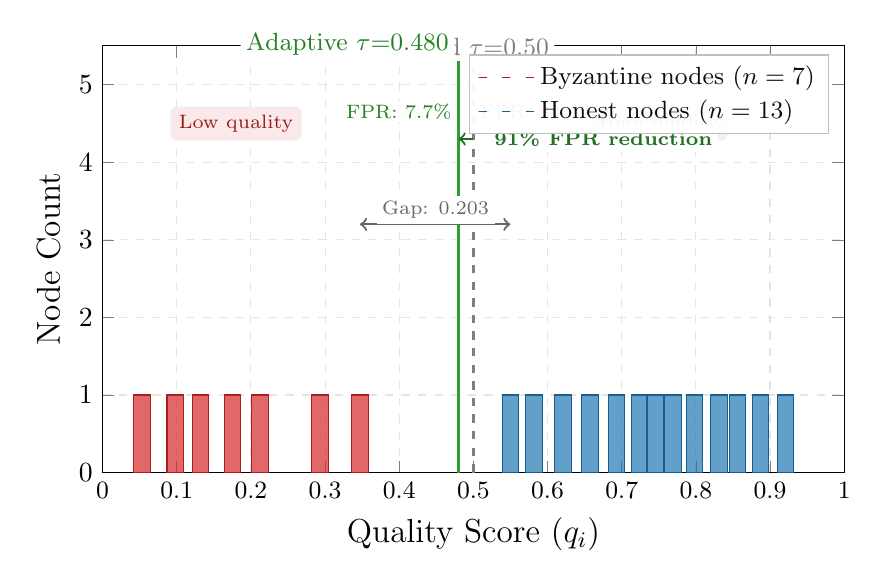
\begin{tikzpicture}
\begin{axis}[
    width=11cm,
    height=7cm,
    xlabel={Quality Score ($q_i$)},
    ylabel={Node Count},
    xlabel style={font=\large},
    ylabel style={font=\large},
    xmin=0, xmax=1.0,
    ymin=0, ymax=5.5,
    xtick={0, 0.1, 0.2, 0.3, 0.4, 0.5, 0.6, 0.7, 0.8, 0.9, 1.0},
    xticklabel style={font=\small},
    ytick={0,1,2,3,4,5},
    grid=both,
    grid style={dashed, gray!20},
    legend style={
        at={(0.98,0.98)},
        anchor=north east,
        font=\small,
        draw=gray!50,
        fill=white,
        fill opacity=0.95,
    },
    legend cell align=left,
    clip=false,
]

% Byzantine nodes quality scores (sign flip, 35% BFT = 7 nodes)
% Scores: 0.053, 0.098, 0.132, 0.175, 0.212, 0.293, 0.347
% Represented as histogram-like vertical bars
\addplot[ybar, bar width=6pt, fill=byzantinered, fill opacity=0.7, draw=byzantinered!80!black]
coordinates {
    (0.053, 1) (0.098, 1) (0.132, 1) (0.175, 1) (0.212, 1) (0.293, 1) (0.347, 1)
};
\addlegendentry{Byzantine nodes ($n=7$)}

% Honest nodes quality scores (13 nodes)
% Scores clustered around 0.55-0.92
\addplot[ybar, bar width=6pt, fill=honestblue, fill opacity=0.7, draw=honestblue!80!black]
coordinates {
    (0.550, 1) (0.582, 1) (0.621, 1) (0.657, 1) (0.693, 1) (0.724, 1)
    (0.745, 1) (0.769, 1) (0.798, 1) (0.831, 1) (0.856, 1) (0.887, 1) (0.921, 1)
};
\addlegendentry{Honest nodes ($n=13$)}

% Fixed threshold at 0.5 (bad: catches 11 of 13 honest nodes)
\draw[fixedgray, very thick, dashed] (axis cs:0.5, 0) -- (axis cs:0.5, 5.3);
\node[font=\small, fixedgray, fill=white, inner sep=2pt, rounded corners=1pt, anchor=south]
    at (axis cs:0.5, 5.3) {Fixed $\tau{=}0.50$};
\node[font=\scriptsize, byzantinered!80!black, fill=white, inner sep=1pt, anchor=north west]
    at (axis cs:0.505, 4.8) {FPR: 84.6\%};

% Adaptive threshold at 0.48 (good: 0% FPR)
\draw[adaptivegreen, very thick] (axis cs:0.480, 0) -- (axis cs:0.480, 5.3);
\node[font=\small, adaptivegreen!80!black, fill=white, inner sep=2pt, rounded corners=1pt, anchor=south east]
    at (axis cs:0.475, 5.3) {Adaptive $\tau{=}0.480$};
\node[font=\scriptsize, adaptivegreen!80!black, fill=white, inner sep=1pt, anchor=north east]
    at (axis cs:0.475, 4.8) {FPR: 7.7\%};

% Gap annotation
\draw[<->, thick, black!60] (axis cs:0.347, 3.2) -- (axis cs:0.550, 3.2);
\node[font=\scriptsize, black!60, fill=white, inner sep=2pt, anchor=south]
    at (axis cs:0.449, 3.2) {Gap: 0.203};

% Region annotations
\node[font=\scriptsize, byzantinered!70!black, fill=byzantinered!10, inner sep=3pt, rounded corners=2pt]
    at (axis cs:0.18, 4.5) {Low quality};
\node[font=\scriptsize, honestblue!70!black, fill=honestblue!10, inner sep=3pt, rounded corners=2pt]
    at (axis cs:0.75, 4.5) {High quality};

% 91% improvement annotation
\draw[->, thick, adaptivegreen!70!black] (axis cs:0.5, 4.3) -- (axis cs:0.48, 4.3);
\node[font=\scriptsize\bfseries, adaptivegreen!70!black, fill=white, inner sep=2pt, anchor=west]
    at (axis cs:0.52, 4.3) {91\% FPR reduction};

\end{axis}
\end{tikzpicture}
\end{document}
